\documentclass[11pt]{article}
\usepackage[T1]{fontenc}
\usepackage[utf8]{inputenc}
\usepackage{lmodern}
\usepackage{amsmath,amssymb,amsthm,mathtools}
\usepackage{microtype}
\usepackage{geometry}
\usepackage{hyperref}
\usepackage{graphicx}
\geometry{margin=1in}

\newtheorem{theorem}{Theorem}
\newtheorem{proposition}{Proposition}
\newtheorem{remark}{Remark}

\newcommand{\N}{\mathbb{N}}
\newcommand{\T}{\mathrm{T}}

\title{Asymptotically Harmonic Partitions of the Harmonic Series}
\author{Vencislav Popov \\
Department of Psychology, University of Zurich \\
\texttt{vencislav.popov@gmail.com}}
\date{\today}

\begin{document}
\maketitle

\begin{abstract}
We arrange the positive integers in a triangular array and sum reciprocals down columns. Each column gives a convergent reciprocal series with strictly convex denominators. If $S^{(k)}$ denotes the $k$th column sum, then the harmonic series decomposes as
\[
\sum_{n=1}^{\infty} \frac{1}{n} = \sum_{k=1}^{\infty} S^{(k)},
\]
while the column sums themselves satisfy $S^{(k)} > 2/k$ for every $k$ and in fact $S^{(k)} \sim 2/k$. This yields a self-similar proof that the harmonic series diverges. This note presents a novel triangular-column variant of the harmonic series divergence proof, adding a structurally distinct approach to the classical literature.
\end{abstract}

\section{Introduction}

The harmonic series
\[
\sum_{n=1}^{\infty} \frac{1}{n}
\]
is one of the standard examples in analysis, and its divergence has been proved in many different ways. Kifowit and Stamps give a very nice survey of such proofs, ranging from Oresme's classical grouping argument to several contradiction proofs, including one based on triangular-number blocks and another family obtained by grouping terms into twos, threes, fours, and so on \cite{KifowitStamps}. That survey is hard to improve upon as a catalog of entertaining arguments.

The present note arose from a simple question: what happens if one takes the triangular-number proof and turns it sideways? The answer is unexpectedly pleasant. Instead of grouping the harmonic series \emph{by rows}, one can decompose it \emph{by columns}. Each column turns out to be a convergent reciprocal series with strictly convex denominators, while the sequence of column sums is itself asymptotically harmonic. This leads to an elegant self-referential proof of divergence: the harmonic series breaks into convergent layers whose total masses again behave like a harmonic series.

\section{The triangular array}

Let
\[
\T_m := \frac{m(m+1)}{2}, \qquad m \ge 0,
\]
with the convention $\T_0=0$. Arrange the positive integers in rows of lengths $1,2,3,\dots$:
\[
\begin{matrix}
1\\[2pt]
2 & 3\\[2pt]
4 & 5 & 6\\[2pt]
7 & 8 & 9 & 10\\[2pt]
11 & 12 & 13 & 14 & 15\\[2pt]
\vdots
\end{matrix}
\]
Thus row $m$ consists of the integers
\[
\T_{m-1}+1,\, \T_{m-1}+2,\, \dots,\, \T_m,
\]
for $m \ge 1$. For each fixed $k \in \N$, let $S^{(k)}$ be the sum of reciprocals down the $k$th column. Since the $k$th column begins in row $k$, we have
\begin{equation}\label{eq:Sk-def}
S^{(k)} := \sum_{m=k}^{\infty} \frac{1}{\T_{m-1}+k}.
\end{equation}
The first few examples are
\[
S^{(1)} = 1 + \frac12 + \frac14 + \frac17 + \frac1{11} + \cdots,
\]
\[
S^{(2)} = \frac13 + \frac15 + \frac18 + \frac1{12} + \frac1{17} + \cdots,
\]
\[
S^{(3)} = \frac16 + \frac19 + \frac1{13} + \frac1{18} + \cdots.
\]

Since every positive integer appears exactly once in the triangular array, these column series partition the harmonic series.

\begin{proposition}\label{prop:partition}
One has
\[
\sum_{n=1}^{\infty} \frac{1}{n} = \sum_{k=1}^{\infty} S^{(k)}.
\]
\end{proposition}

\begin{proof}
The sets of denominators appearing in the columns are pairwise disjoint and their union is $\N$. Since all terms are positive, the identity follows simply by regrouping terms according to their column index.
\end{proof}

\section{Convex denominator sequences}

The first column is
\[
1,2,4,7,11,16,\dots,
\]
which is the minimal strictly convex increasing sequence of natural numbers, namely
\[
a_n = 1 + \frac{n(n-1)}{2}.
\]
More generally, every column has strictly convex denominators.

\begin{proposition}\label{prop:convex}
Fix $k \ge 1$. The denominators in $S^{(k)}$ are
\[
d_m^{(k)} := \T_{m-1}+k \qquad (m \ge k),
\]
and satisfy
\[
d_{m+1}^{(k)} - d_m^{(k)} = m, \qquad d_{m+2}^{(k)} - 2d_{m+1}^{(k)} + d_m^{(k)} = 1.
\]
In particular, each column is a convergent reciprocal series with strictly convex denominators.
\end{proposition}

\begin{proof}
Since $\T_m-\T_{m-1}=m$, the first identity is immediate:
\[
d_{m+1}^{(k)} - d_m^{(k)} = (\T_m+k)-(\T_{m-1}+k)=m.
\]
Taking another difference gives the constant second difference $1$. For convergence, note that $d_m^{(k)} \ge \T_{m-1} \sim m^2/2$, so
\[
\sum_{m=k}^{\infty} \frac{1}{d_m^{(k)}}
\]
converges by comparison with a constant multiple of $\sum m^{-2}$.
\end{proof}

A convenient closed form for the denominators is
\[
\T_{m-1}+k = \frac{m^2-m+2k}{2},
\]
so \eqref{eq:Sk-def} may also be written as
\begin{equation}\label{eq:Sk-rational}
S^{(k)} = \sum_{m=k}^{\infty} \frac{2}{m^2-m+2k}.
\end{equation}
After the index shift $n=m-1$, this becomes
\begin{equation}\label{eq:Sk-shift}
S^{(k)} = \sum_{n=k-1}^{\infty} \frac{2}{n^2+n+2k}.
\end{equation}

\section{A lower bound for the column sums}

The key estimate is pleasantly simple.

\begin{theorem}\label{thm:lowerbound}
For every $k \ge 1$,
\[
S^{(k)} > \frac{2}{k}.
\]
\end{theorem}

\begin{proof}
Starting from \eqref{eq:Sk-shift}, compare the $n$th term with a telescoping one. For $n \ge k-1$,
\[
(n+1)(n+2) - (n^2+n+2k) = 2(n+1-k) \ge 0.
\]
Hence
\[
\frac{2}{n^2+n+2k} \ge \frac{2}{(n+1)(n+2)} = 2\left(\frac{1}{n+1}-\frac{1}{n+2}\right).
\]
Summing from $n=k-1$ to $\infty$ gives
\[
S^{(k)} \ge 2\sum_{n=k-1}^{\infty} \left(\frac{1}{n+1}-\frac{1}{n+2}\right)=\frac{2}{k}.
\]
The inequality is strict because equality holds only for the first term $n=k-1$; for all $n \ge k$ one has $2(n+1-k)>0$.
\end{proof}

\section{A self-similar proof of divergence}

The previous theorem immediately gives a contradiction proof.

\begin{theorem}\label{thm:divergence}
The harmonic series diverges.
\end{theorem}

\begin{proof}
Assume for contradiction that
\[
\sum_{n=1}^{\infty} \frac{1}{n} = M
\]
for some finite $M$. By Proposition \ref{prop:partition},
\[
M = \sum_{k=1}^{\infty} S^{(k)}.
\]
By Theorem \ref{thm:lowerbound},
\[
\sum_{k=1}^{\infty} S^{(k)} > \sum_{k=1}^{\infty} \frac{2}{k}.
\]
Under the assumption that the harmonic series converges to $M$, the right-hand side equals $2M$. Therefore
\[
M > 2M,
\]
a contradiction.
\end{proof}

A compelling feature of this proof is that the harmonic series is decomposed into convergent pieces, but the sequence of their total masses is still large enough to dominate a constant multiple of the harmonic series itself.

\section{Asymptotics}

In fact, the lower bound of Theorem \ref{thm:lowerbound} is asymptotically sharp.

\begin{proposition}\label{prop:asymptotic}
As $k \to \infty$,
\[
S^{(k)} \sim \frac{2}{k}.
\]
\end{proposition}

\begin{proof}
The lower bound $S^{(k)} > 2/k$ is already known. For an upper bound, split off the first term in \eqref{eq:Sk-shift} and then compare the remaining denominator with $n(n+1)$:
\[
S^{(k)} = \frac{2}{k(k+1)} + \sum_{n=k}^{\infty} \frac{2}{n^2+n+2k}
< \frac{2}{k(k+1)} + \sum_{n=k}^{\infty} \frac{2}{n(n+1)}.
\]
Since
\[
\sum_{n=k}^{\infty} \frac{2}{n(n+1)} = \frac{2}{k},
\]
we obtain
\[
\frac{2}{k} < S^{(k)} < \frac{2}{k} +  \frac{2}{k(k+1)} 
\]
The error term is $O(k^{-2})$, so $S^{(k)} = \frac{2}{k} + O(k^{-2})$, and in particular $S^{(k)} \sim \frac{2}{k}$.
\end{proof}

Thus the harmonic series admits a decomposition into convergent convex subseries whose total masses are themselves asymptotically harmonic.

\section{A few remarks and variants}

\begin{remark}
The first column sum is
\[
S^{(1)} = 1 + \frac12 + \frac14 + \frac17 + \frac1{11} + \cdots = \sum_{n=1}^{\infty} \frac{1}{1+\frac{n(n-1)}{2}}.
\]
A short calculation with partial fractions and the digamma function yields the pleasant closed form
\[
S^{(1)} = \frac{2\pi}{\sqrt{7}}\tanh\!\left(\frac{\pi\sqrt{7}}{2}\right) \approx 2.3736546754.
\]
So the largest column sum is already finite and quite small.
\end{remark}

\begin{figure}[t]
\centering
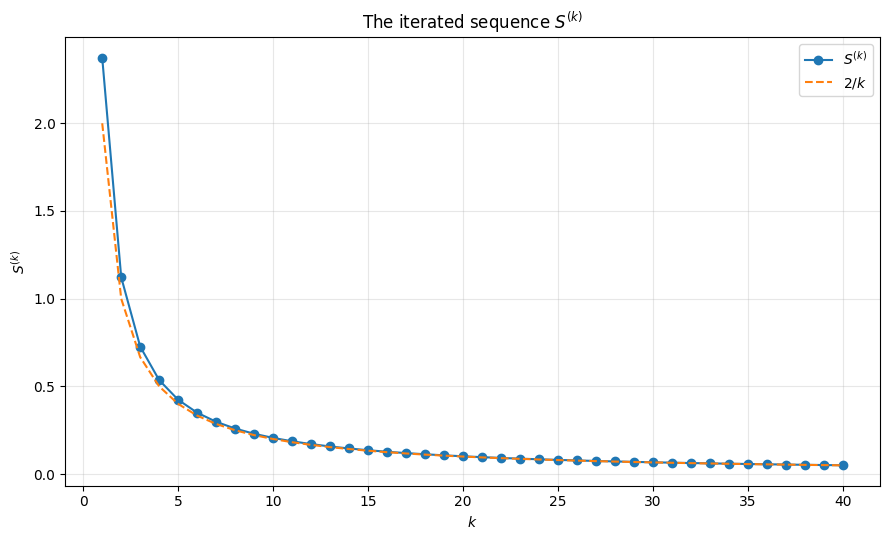
\includegraphics[width=0.8\linewidth]{Sk_plot}
\caption{The column sums $S^{(k)}$ plotted against $k$, with the asymptotic curve $2/k$ overlaid. The sequence drops quickly and then tracks $2/k$ closely, consistent with the asymptotic relation $S^{(k)} \sim 2/k$. The first few values are $S^{(1)} \approx 2.37365$, $S^{(2)} \approx 1.12229$, $S^{(3)} \approx 0.72680$, and $S^{(4)} \approx 0.53564$.}
\label{fig:Sk-asymptotic}
\end{figure}

\begin{remark}[Closed forms for the column sums]
More generally, for every \(k \ge 1\),
\[
S^{(k)}
=
\sum_{m=k-1}^{\infty} \frac{2}{m^2+m+2k}.
\]
By separating off the first \(k-1\) terms from the full series, one obtains for \(k \ge 2\)
\[
S^{(k)}
=
\frac{2\pi}{\sqrt{8k-1}}
\tanh\!\left(\frac{\pi\sqrt{8k-1}}{2}\right)
-
2\sum_{m=0}^{k-2}\frac{1}{m^2+m+2k}.
\]
Equivalently, writing \(\psi\) for the digamma function and \(\Im\) for the imaginary part,
\[
S^{(k)}
=
\frac{4}{\sqrt{8k-1}}
\Im \psi\!\left(k-\frac12+\frac{i\sqrt{8k-1}}{2}\right).
\]
Thus each column sum can be written explicitly, and the first few values are
\[
S^{(1)} \approx 2.37365,\qquad
S^{(2)} \approx 1.12229,\qquad
S^{(3)} \approx 0.72680,\qquad
S^{(4)} \approx 0.53564.
\]
While these closed forms are not needed for the divergence argument, they reinforce the sense that the triangular decomposition has a surprisingly rigid and explicit structure.
\end{remark}

\begin{remark}
There is a close family resemblance between the present argument and several proofs discussed by Kifowit and Stamps \cite{KifowitStamps}. In particular:
\begin{itemize}
    \item their Proof~6 is a contradiction proof obtained by grouping the harmonic series into pairs, with the remark that analogous arguments arise from grouping in threes, fours, and so on;
    \item their Proof~13 uses a telescoping decomposition to derive a contradiction of the form $S=1+S$;
    \item their Proof~14 groups the harmonic series by triangular-number rows and obtains the contradiction $S>2(S-1)$.
\end{itemize}
While the present note shares a family resemblance with these grouping arguments, its vertical, column-wise partition offers a structurally distinct perspective.
\end{remark}

\section{Conclusion}

The triangular array of positive integers carries two natural directions. Reading by rows gives one of the classical triangular-number proofs of the divergence of the harmonic series. Reading by columns gives a different picture: one obtains convergent reciprocal series with strictly convex denominators, but their total masses remain harmonically large. The resulting proof highlights an elegant and largely unexplored fractal-like property of the harmonic series.

\begin{thebibliography}{9}

\bibitem{KifowitStamps}
S.~J.~Kifowit and T.~A.~Stamps,
\emph{The Harmonic Series Diverges Again and Again},
The AMATYC Review, Spring 2006.

\end{thebibliography}

\end{document}